\documentclass[10pt]{article}
\usepackage[margin=1in]{geometry}
\usepackage{graphicx}
\usepackage{amsmath}
\usepackage{xcolor}
\usepackage[colorlinks=true, linkcolor=blue]{hyperref}
\graphicspath{{figs/}}
\title{Pilot-Proxy Findings Ledger\\
\large A living supplement of dissertation-grade results behind the RASTI article}
\author{D.~Gormley}
\date{Started 2026 July 18 --- updated with each round}

\begin{document}
\maketitle

\noindent\emph{Purpose.} The RASTI article keeps only what its argument
needs. This ledger keeps the rest: measured findings, methodological
lessons, and negative results that belong in the dissertation's
narrative even where the article compresses them to a clause. Every
number here maps to a command in the public repository or an archived
provenance memo; sections cite the source. The full supplementary plot
set (all-23 spectra in three variants, per-channel $F$ distributions,
diurnal and stratified diagnostics) travels separately as
\texttt{supplemental\_plots\_rev16.zip}.

\section{ch30 dissected: transmitter silences, not fades}
\label{s:ch30}
The refused channel ch30 is cleanly bimodal (Fig.~\ref{f:ch30}): 96.3
per cent of frames sit in a tight clump at $11.7\times\mu_0$, the range
$1.5$--$10\times\mu_0$ is essentially empty (0.26 per cent), and a 3.46
per cent minority (314 frames) sits below. The minority is 38
\emph{whole} captures --- not one capture mixes the two populations ---
confined to 2019 April 6--25 plus one day in October. That structure
rules out propagation fades: the dominant occupant simply went off the
air, twice, in 2019, and never again in 7.6 years of sampled exposure.
The census makes the attribution nearly forced: CHKL-1 (Relay,
Penticton BC) sits 17.7\,km from DRAO at 79.3\,dB detectability ---
25\,dB clear of the runner-up (CH2520-DT, 156\,km) --- and a 17.7\,km
path never fades into the gap, which is why ch30's mask is effectively
deterministic presence detection. One nuance worth keeping straight:
in our census source the \emph{Relay} class carries a $\pm$1\,kHz
tolerance entry; it is the \emph{translator/LPTV} class that records
none (the ch33 story, \S\ref{s:ch33}). ch30's measured drift picket
across its guard band is therefore evidence of poor carrier discipline
in practice, not of a permissive rule on paper. The off-air interval
is a datable, checkable event (ISED records; pending).

Two more results fall out of the dissection. First, the minority's
centre lies within $1.5\times10^{-3}$ of the \emph{analytic} zero
point: the moment the transmitter goes silent, the channel relaxes to
exactly where the detector model says a clean channel sits --- direct,
per-channel evidence that the refusal is transmitter-caused rather
than instrumental. Second, the minority is \emph{not} a usable
calibration core: within-capture width $37\times10^{-3}$ (fifteen
times the trusted-channel null width), capture means scattered
$18\times10^{-3}$ rms in both directions (weak residual co-channel
energy in target \emph{and} reference cells once the dominant is off),
occupancy 0.5 per cent against the 15 per cent floor. The
mixture-model reclamation route, applied to the one channel that
invites it, confirms the refusal. Repro:
\texttt{analysis/ch30\_offair\_minority.py};
\texttt{ch30\_offair\_minority.csv}.

\begin{figure}[h]
\centering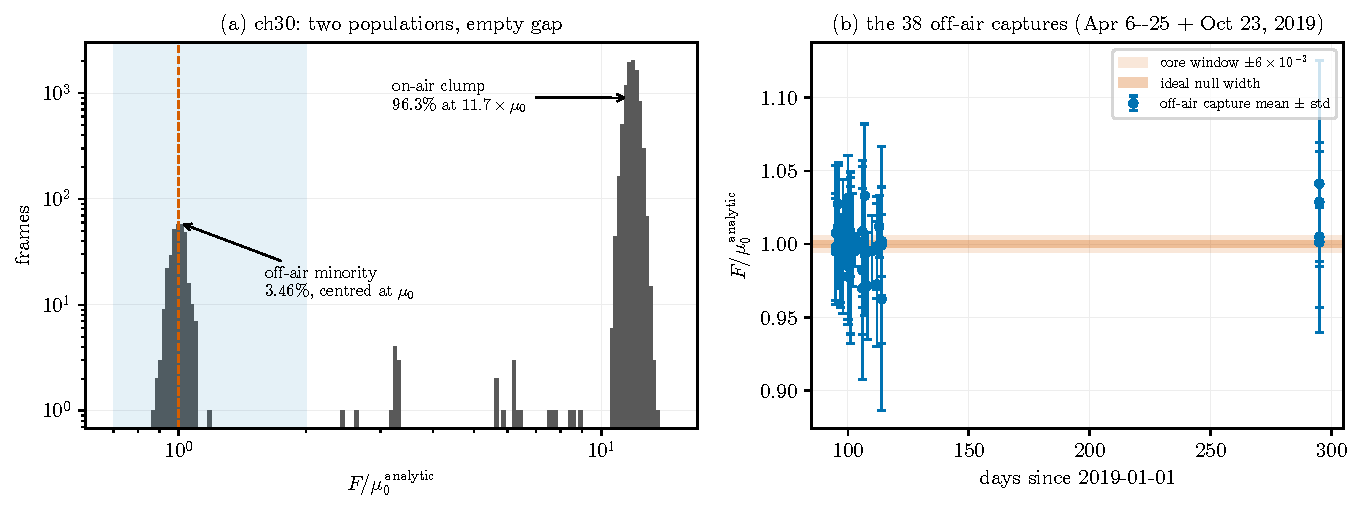
\includegraphics[width=0.95\textwidth]{figS_ch30_two_population}
\caption{ch30's two populations. (a) The on-air clump at
$11.7\times\mu_0$ and the off-air minority at $\mu_0$, with an
essentially empty gap between. (b) The 38 off-air captures: means
within a few $10^{-3}$ of the analytic zero point, but widths far
beyond a true null core.}
\label{f:ch30}
\end{figure}

\paragraph{The ch24 contrast.} The archive's other refusal dies by the
opposite geometry. ch24 has \emph{no} shape to cut: its core is
displaced $+20.4\times10^{-3}$ (signal-elevated by persistent in-cell
carriers), occupancy 7.6 per cent, a continuum rather than a bimodal
split --- there is no gap for a mixture model to exploit. And no more
samples are coming: ch24 is already sampled at full archive depth
(1722 of 1722 events), so the running survey extension adds nothing
there. Only new observations could change its picture, and the
persistent-occupant physics says they would not. The pair makes a tidy
taxonomy: \textbf{ch30 is separable but its null is unusable; ch24 is
unseparable outright.} Both refusals are final on this archive.

The time dissection (Fig.~\ref{f:ch24t}) completes the contrast.
ch24's $F$ never leaves the band $\sim$0.93--1.3$\times\mu_0$
(nothing above 1.3 beyond 0.2 per cent; compare ch30's clump at
11.7), and it is \emph{two-sided}: 26 per cent of frames sit below
$0.99\times\mu_0$, more than $4\sigma$ under the null --- measured
proof that co-channel energy lands in the \emph{reference} cells and
pushes $F$ down, the same mechanism seen on ch30's off-air wings and
the empirical leg of the purity-is-not-monotonic argument
(\S\ref{s:tau}). Against time it is a stationary committee: quarterly
medians hold at 1.02--1.05 from 2018 Q4 through 2026 Q2 with no step,
no repack signature, and no silence --- 4 isolated quiet captures out
of 1722 (0.2 per cent, scattered single days: momentary deep fades,
never a window), versus ch30's 38-capture three-week silence. The
census explains the difference in kind: ch30 is a monolith (one
17.7\,km relay, 25\,dB clear), while ch24's list is led by the
CHKL-DT$+$CHBC-DT channel-share at 62.8\,km with relay and translator
members behind it --- a committee is never all off at once. One
genealogical note worth keeping: CHKL-\emph{DT}, the ch24 share
parent in Kelowna, is the parent station of CHKL-1, the ch30
Penticton relay --- the same broadcast family plausibly occupies both
refused channels (census candidates; ISED corroboration pending), and
the parent shows no interruption during the relay's 2019 April
silence. Sampled-epoch caveat: the ch24 archive itself has coverage
holes (2021--2024 Q2 and 2025 hold no captures) --- an archive
property, not a transmitter property; within every sampled epoch the
committee is stationary.

\begin{figure}[h]
\centering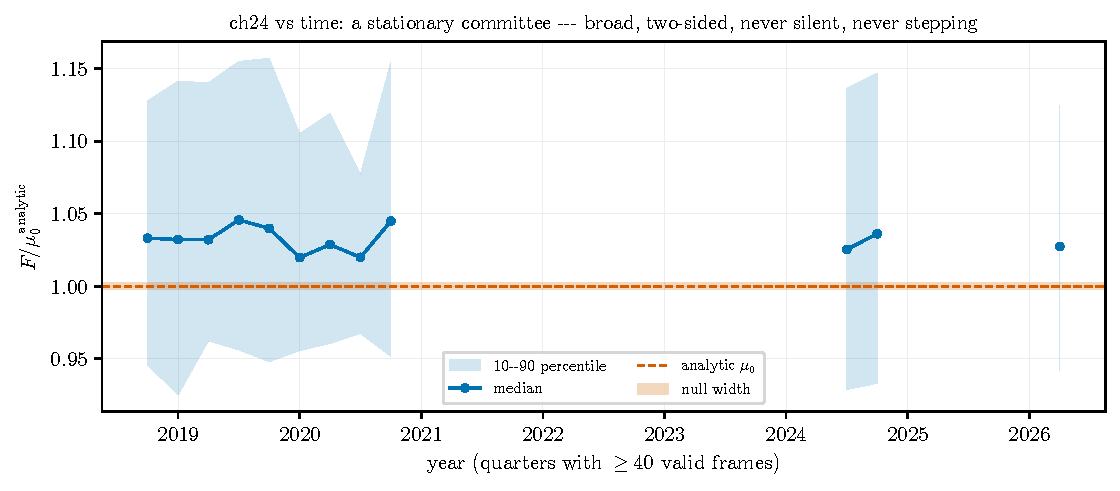
\includegraphics[width=0.9\textwidth]{figS_ch24_vs_time}
\caption{ch24 against time: quarterly median and 10--90 percentile
band of $F/\mu_0$. Broad, two-sided about a displaced core, stationary
across 7.6 years, never silent --- the committee counterpart to
ch30's monolith.}
\label{f:ch24t}
\end{figure}

\section{The T2 saga: a generator startup transient}
\label{s:t2}
The synthetic golden capture's pilot read $\sim$0.5\,dB low against
its own specification, and the deficit \emph{moved} (0.53--0.72\,dB)
depending on which estimator and sample span measured it. The
resolution came from a ten-block coherent projection
(Fig.~\ref{f:t2}): block 0 sits $-9.71$\,dB and block 1 $-0.41$\,dB
below the stationary mean of blocks 2--9 --- the waveform generator
takes $\sim$11\,ms to reach steady state, and every full-span scalar
inherited a diluted average of that ramp. Once cropped to the
stationary span and retrimmed ($\times 0.98447$), two independent
estimators agreed to 0.007\,dB, and the steady-state pilot sits
0.136\,dB \emph{above} nominal. Lessons worth keeping: (i) a
``span-dependent scalar'' is a symptom of non-stationarity, not of a
broken estimator; (ii) the two estimators' 0.194\,dB convention gap
was itself stable through the trim --- measured, predicted, then
closed; (iii) always discard the first $\sim$120k samples at
generation. Provenance:
\texttt{data/provenance/t2\_convention\_20260718/};
\texttt{T2\_RESOLUTION} and R9/R10 triage memos.

\begin{figure}[h]
\centering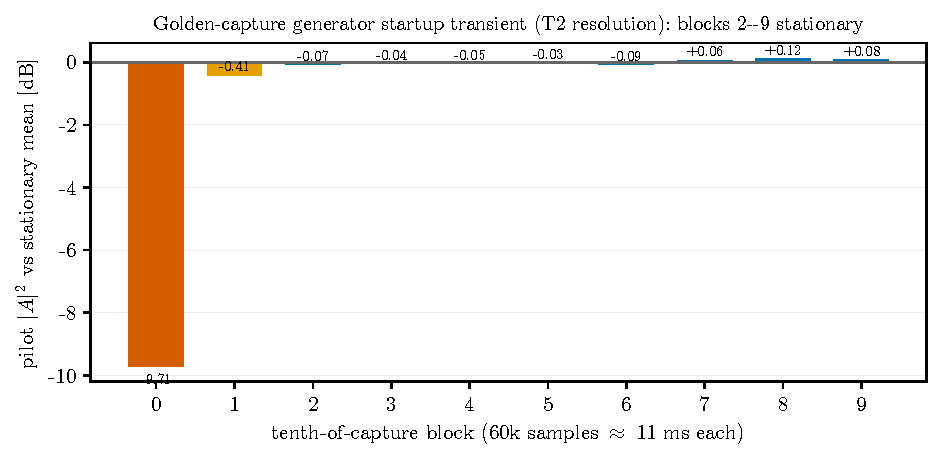
\includegraphics[width=0.72\textwidth]{figS_t2_block_profile}
\caption{The T2 resolution in one picture: the golden capture's pilot
power by tenth-of-file block. The deficit was never in the detector
--- it was the generator warming up.}
\label{f:t2}
\end{figure}

\section{A falsified physics alternative}
The one mechanistic model we built for the zero-point shifts --- the
aliased-noise gain of the 4-tap sinc-Hamming reference PFB prototype
through the $K{=}128$ window --- \emph{fails}: it predicts $-1.8$ to
$-4.2\times10^{-3}$ for the near-edge channels 18/29/32/35, where the
measurement is consistent with zero, and captures only a third of
ch21's $-12\times10^{-3}$ wrap shift
(\texttt{fig\_pfb\_zero\_point\_prediction}). The deployed F-engine
coefficients evidently differ from the reference prototype. The
dissertation-grade point: we kept the falsification in the paper and
let the measured 23-entry table be the calibration --- ``the measured
table, not a mechanism'' is an honest and defensible calibration
philosophy when the deployed instrument diverges from its
documentation.

\section{From magic numbers to a derived criterion}
The null-core trust flags began life as placeholders (0.9 mask
fraction, 15 per cent occupancy, $20\times10^{-3}$ range). They ended
as one derived criterion measured two ways plus a geometry bound:
because the positive-excess rule masks null frames at 0.5 by
construction, a mask fraction $>0.9$ \emph{is} the statement
$f_{\rm null} = 2(1-\mathrm{mf}) < 0.2$; the core-window occupancy
floor is the same $f_{\rm null}$ by direct count (the
$\pm 6\times10^{-3}$ window is 2.5 ideal null widths); and the
displacement bound $20\times10^{-3}$ is $1.7\times$ the largest
geometry-producible shift (ch21's wrap). The archive then shows the
constants are not delicate: trusted channels sit at occupancy
$\ge 19.5$ per cent and $|$gap$| \le 12\times10^{-3}$; refused ones at
$\le 7.6$ per cent and $\ge 20.4\times10^{-3}$. Bimodal separation is
what makes a threshold criterion robust --- the same structural fact,
twice, at two scales of the analysis (cf.\ \S\ref{s:ch30}).

\section{The width-crossing scale and its universal curve}
The detector's sensitivity has a natural unit: the shelf SNR $s$ at
which the induced mean shift $C\,s$ equals the null width
$\sigma = \sqrt{1/R + 1/2R}$. In the reduced variable
$k = C s/\sigma$, the detection probability collapses onto one curve
across dimensionalities --- $P_d(k{=}1) = 0.833$ at $-34.30$\,dB for
512-row trials and $0.841$ at $-47.85$\,dB for full frames ---
so ``per-trial'' and ``deployment-scale'' quotes are the same physics
at different $R$. The flip side is a universal caveat the tiering
must carry: signal below the width crossing retains at $\approx$0.5 on
\emph{every} channel by construction. Sensitivity claims and
retention claims are two readings of one number.

\section{Why the threshold sits at the mean, not deeper in the left tail}
\label{s:tau}
The natural challenge to $\tau = \hat\mu_0$ is: if kept data must be
clean, why not keep only the far left tail? The quantitative answer
(Fig.~\ref{f:tau}) is that the null and a weak-signal population are
the \emph{same distribution shifted by} $k\sigma$, so a deeper cut
buys purity only at the Gaussian hazard exchange rate --- and pays for
it exponentially in exposure. Moving the threshold from the mean to
$2\sigma$ below it keeps 2.3 per cent of clean frames instead of 50
per cent ($22\times$ less data, $4.7\times$ worse map noise for fixed
survey time), while the contamination \emph{fraction} of what is kept
improves by only $1.2\times$ for sub-width signal at $k=0.1$,
$1.6\times$ at $k=0.3$, and $5.4\times$ even at the width crossing
$k=1$. Below the width crossing --- the only regime a deeper cut is
supposed to protect --- both thresholds retain signal at nearly the
null rate, so the purity of kept data barely moves: you cannot
tail-cut your way out of $k \ll 1$. What actually bounds that regime
is the measurement program (pilot-free floor, injection retention
curve, veto arm, per-channel occupancy priors), which pays linearly
rather than exponentially.

Four further properties select the mean exactly. (i) It is the one
threshold requiring \emph{no width calibration}: $\hat\mu_0$ is the
best-measured point of the distribution (mode-anchored median,
$\sim 3\times10^{-5}$ error), while any tail threshold inherits the
per-channel width, which carries no assigned uncertainty. (ii)
Symmetry makes the null keep-fraction exactly $1/2$, which is what
turns the mask fraction into a free, continuous health check ---
binomial sensitivity is maximal at 0.5, and a drift test at a 2.3 per
cent keep rate would need hundreds of times the frames. (iii) It is
parameter-free: $P_d(k) = \Phi(k)$ with no engineered constant ---
$\Phi(1) = 0.84$ is the measured 0.833/0.841 --- so the whole
validation chain anchors to it. (iv) Purity is \emph{not} monotonic
in depth in this system: anything that adds power to the reference
cells pushes $F$ \emph{down} (measured on ch30's off-air captures,
whose means scatter both ways), so frames far below the mean carry
\emph{enhanced} odds of reference-side contamination --- the band
floor exists precisely because low $F$ is not clean $F$. The kept set
is therefore a window, $[\hat\mu_0 - 5\sigma,\ \hat\mu_0]$: the
entire trustworthy part of the left tail, cut at the point where
every one of these arguments meets.

\begin{figure}[h]
\centering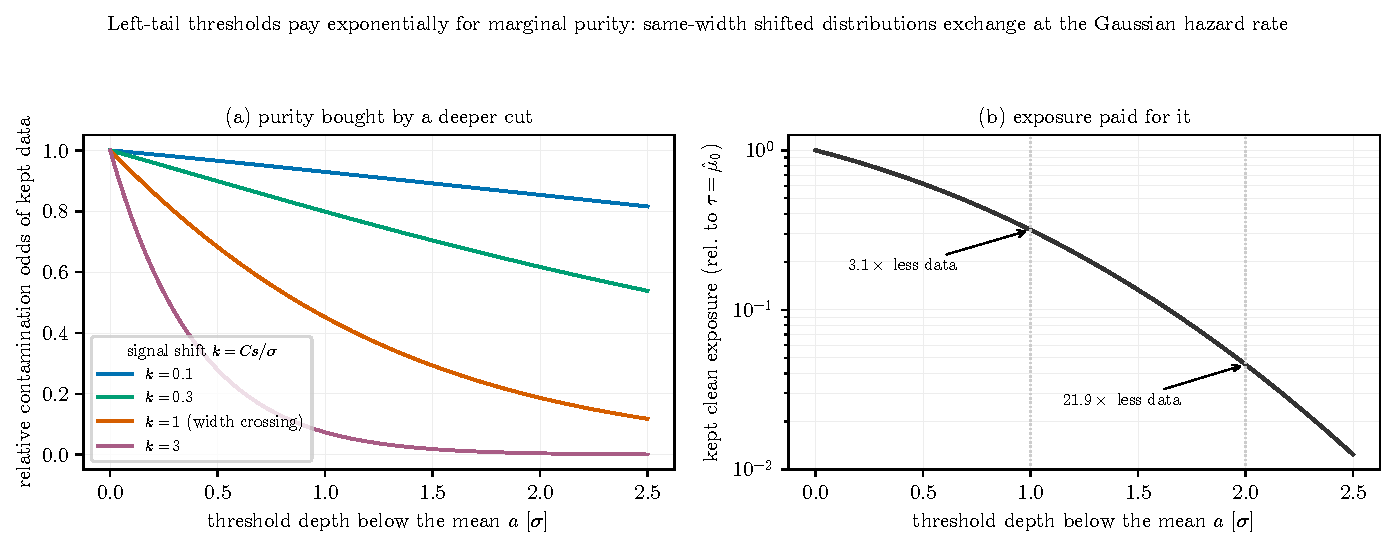
\includegraphics[width=0.97\textwidth]{figS_threshold_exchange}
\caption{The exchange rate of left-tail thresholds: purity gain per
kept frame (a) against clean exposure surrendered (b), for signal
shifts $k$ in null widths. The deep tail pays $22\times$ in data for
$1.2$--$1.6\times$ in purity against sub-width signal.}
\label{f:tau}
\end{figure}

\paragraph{Recorded options, deliberately not engineered now.} Three
design notes ratified 2026-07-18, kept for the future rather than
built: (1) the per-channel zero-point offsets map to per-channel
$P_d$ statements through the Fig.-3 meter --- worth an explicit
exposition (``how the offset moves $P_d$'') when presenting; (2)
re-centring a channel's target weight onto a measured off-nominal
carrier (the ch33 option, already recorded in the article) remains a
constants-level change within existing machinery; (3) threshold
self-calibration: the kernel's exact num/den readback supports
continuous per-channel $F$-histogram accumulation, so the measured
table could regenerate as an automated slow loop with atomic
constant swaps ($\sim$2M frames/channel/day at 23.8 frames/s ---
one day of deployment exceeds the whole archive's per-channel
statistics) with the same trust flags refusing contaminated
calibrations. All three are recorded to avoid pre-deployment
over-engineering, not because they are hard. A fourth, recorded
2026-07-18 from Dylan's recollection of fid 552: ch33's occupant may
be a \emph{drifting} oscillator (tracked 2019--2023 in prior CHIME
monitoring). The per-frame cells already corroborate cell-crossing in
the loud era --- quarterly low-tail rates of 13--29 per cent through
2018--2020 (reference-cell power depressing $F$) against a uniform
2.3--5.4 per cent from late 2022, interleaved with the 33--47 per
cent detection spikes --- reading as an oscillator wandering across
the lower reference, guard, and target cells before settling in the
guard, where the two accumulated lines would be dwell positions
(ch30-picket morphology). If confirmed, this is an alternative
mechanism for the 2020 rate collapse (walked out of the cells, vs
departed in the repack) and would kill the departed-occupant-ghost
reading of the blind spot. A 36-event targeted spectra job
(\texttt{ch33\_drift\_events.txt},
\texttt{ch33\_drift\_spectra.py}; one event per quarter, three
through the transition, 640 frames, CPU-only, batch-resumable) is
prepared and deferred pending the survey extension.

\section{Secular transitions, the repack, and a dilution lesson}
Seven years of per-frame rates resolve transmitter history directly
(\texttt{fig\_secular\_rates}): ch33 collapses $\sim$40 to $\sim$4 per
cent by 2020 Q2 (repack-consistent); ch32 falls $\sim$35 to $<$1 per
cent in 2023 April--May (monthly: 0.36, 0.30, 0.09, 0.005); ch35
switches on to $\sim$17 per cent in 2021 Q4 --- eighteen months after
CBUT's confirmed 2020-05-01 repack move, which is itself a puzzle
(interim vs full facility); ch17 rises $\sim$5 to $\sim$35 per cent
across the baseline. All four persist in the classified-FRB stratum
(\texttt{fig\_secular\_frb\_stratum}), so archive composition does not
manufacture them. Two additions came from pushing the scan to
\emph{every} calibrated channel: ch34's step (3--8 per cent through
2020 $\rightarrow$ $\approx$2 $\rightarrow$ $\approx$1) hides below
the episodic membership criterion because a full-period tail fraction
\emph{dilutes} any epoch that is short against total exposure --- a
general lesson about full-period selection criteria --- and ch27
carries a 38 per cent sampled interval in 2020 Q3 with its interior
unsampled. Also worth remembering: the newest quarter (2026 Q2) shows
an all-events-elevated / FRB-flat signature on several channels
simultaneously --- the same compositional artifact as ch33's spurious
2020 Q4 ``rebound.'' Rate structure you cannot reproduce inside a
uniform trigger class is not transmitter history.

\section{ch33: the silent blind spot and the loose-tolerance class}
\label{s:ch33}
ch33 is the channel every per-frame diagnostic scores as clean ---
trusted calibration, $\approx$0.5 mask fraction, zero measured leak
--- and that is precisely the hazard: its only extracted carriers sit
in the skipped guard ($-3.6$\,kHz at 21\,dB integrated SNR), where the
detector's response is $-17$\,dB. ``Clean'' and ``blind'' are
indistinguishable from inside the statistic. The taxonomy that came
out of this is the risk framing the whole deployment section leans
on: a strong co-channel station \emph{on} the nominal pilot is
maskable and costs exposure only (ch24, ch30); an \emph{off-nominal}
pilot is DTV the mask responds to only weakly and rides into kept
data. The census ties the hazard to a licensing class: translator/LPTV
entries carry no frequency-tolerance value in the source, and ch33's
census holds 11 such loose-tolerance candidates within 500\,mi
(\texttt{fig1\_census\_context}). Whether the guard carrier is the
current translator or the integrated ghost of the departed pre-repack
occupant awaits the epoch-split accumulation --- one of the cleanest
open questions the dissertation can pose.

\section{Instrument tones: marked, justified, and how wide to cut}
\label{s:tones}
Of six narrow lines found outside the detector cells across all 23
channels (Fig.~\ref{f:tones}), five sit within 9.5\,Hz --- less than
half a spectral bin --- of $\pm f_s/5$, $\pm f_s/3$, $\pm 2f_s/5$ in
baseband ($f_s = 390.625$\,kHz). The per-tone case for excision rests
on three independent legs, each visible in the gallery: (i) the
\emph{arithmetic} coincidence with rational clock fractions, at
odds of order $10^{-3}$ per line by chance; (ii) each line lives in
exactly one coarse channel, as chain-specific digital spurs do and as
broadcast signals do not; (iii) the prominence is unchanged
($|\Delta| \le 0.3$\,dB) when the analytic mask removes roughly half
the frames --- a sky signal correlated with DTV presence could not be
mask-invariant. The sixth line (ch17, $+157.285$\,kHz) matches no
fraction and is deliberately \emph{retained}: unidentified means
unexcised. All six sit $\ge$73.6\,kHz (24 fine bins) from any
detector-cell support, so excision is cosmetic for the statistic
either way --- notches touch only the supplementary plotting copies.

The notch width itself became a measurement (Dylan's catch,
2026-07-18): a fixed $\pm$3-bin pad left residual skirts of $+2.3$\,dB
(ch14), $+4.4$\,dB (ch29, whose feature is 7 bins wide before
skirts), and $+2.1$\,dB (ch34) outside the cut, while the narrow
$f_s/3$ pair (ch25/28) was clean. The fix is an adaptive notch that
grows from the detected group until the spectrum falls within
0.5\,dB of the local background (bounded at $\pm$15 bins, then
$+$3-bin pad), giving extents of $\pm$8 (ch14), $\pm$13 (ch29), and
$\pm$9 (ch34) bins --- re-audited: no residual above 1\,dB anywhere.
Lesson worth keeping: spur \emph{skirts} scale with spur strength, so
a one-size pad under-cuts exactly the lines that matter most.

\begin{figure}[h]
\centering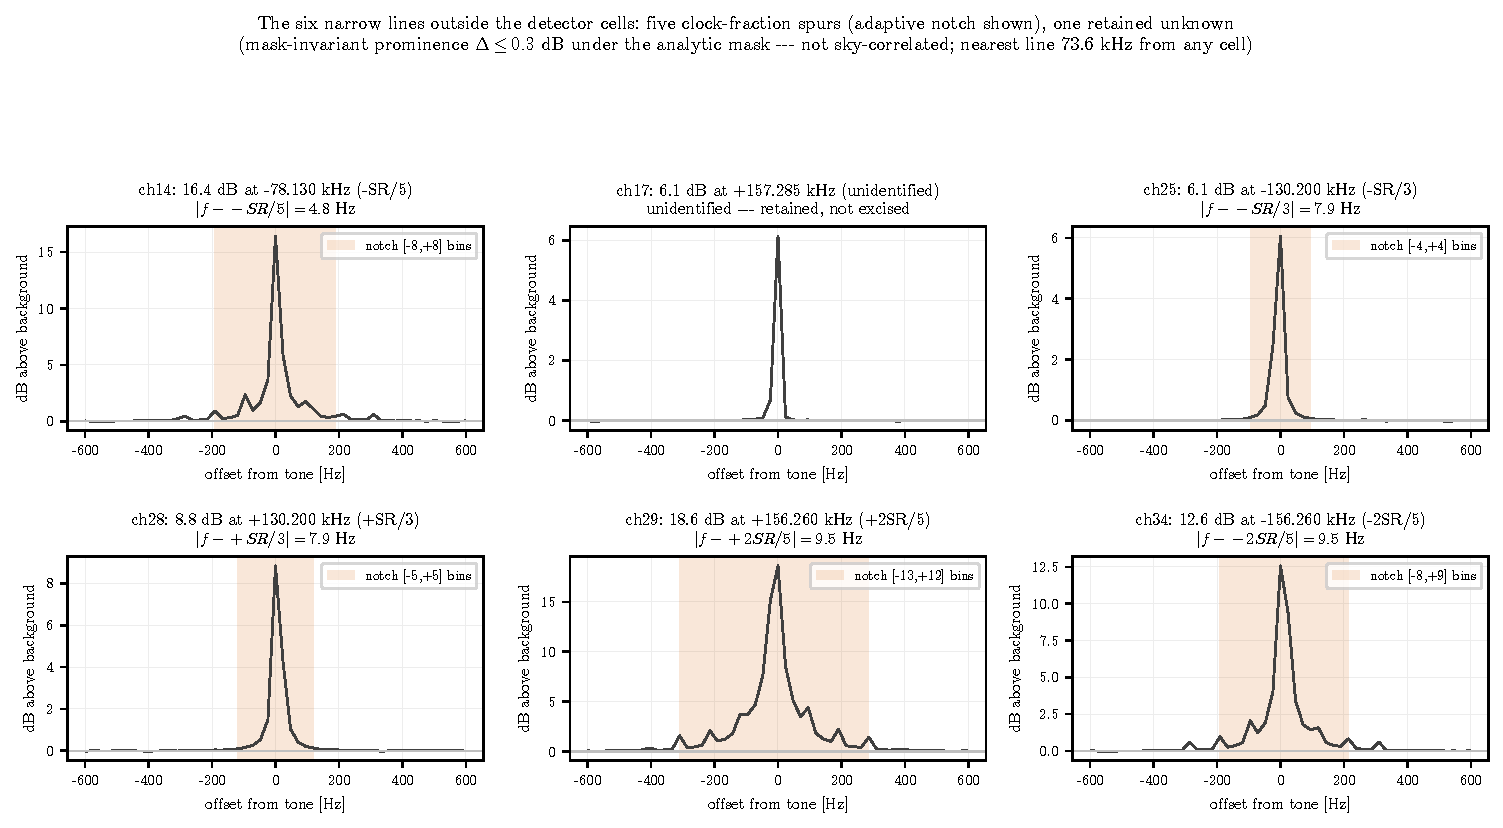
\includegraphics[width=\textwidth]{figS_tone_gallery}
\caption{The instrument-tone gallery: every narrow line outside the
detector cells, marked and identified, with the adaptive notch extent
shaded. The ch17 unknown is retained, not excised.}
\label{f:tones}
\end{figure}

\section{Off-nominal lines vs the census: verified, not assumed}
After instrument-tone removal, four channels retain extracted lines
outside their target cells. ``Rogue transmitters'' was the working
assumption; the census check makes it a verification. Every one of
the four has loose-tolerance candidates licensed on that channel:
ch24 ($+3121$\,Hz at 8\,dB; 3 relays $+$ 12 translators, nearest
K24LM-D at 146\,km), ch30 (the drift picket --- four lines at
$-3899$/$-3494$/$+3110$/$+3611$\,Hz, 8--10\,dB each, spanning both
guards; nearest candidate CHKL-1 itself at 18\,km, and four dwell
positions of one wandering carrier integrated over years is the
economical reading), ch31 ($-2283$\,Hz at 7\,dB; 3 relays $+$ 17
translators, nearest 79\,km), and ch33 ($-3606$/$-2843$\,Hz at
21/13\,dB; 1 relay $+$ 9 translators, nearest K33NM-D at 101\,km).
No channel shows an off-nominal line with an empty candidate list ---
the transmitter hypothesis survives everywhere. The ch33 nuance is
the honest residual: its nearest loose candidate is 101\,km out, so
unlike ch30 the attribution is not forced to a single station, and
the current-translator-vs-departed-occupant question stays open until
the epoch-split accumulation.

\section{Survey forensics: joining 77k captures to their events}
The archive's capture units carry only timestamps; the inventory
carries only day-level dates and classes. The join that made the
stratified analysis possible is (day $\pm$1, unit frame count $=$
$\lfloor$inventory $n_{\rm frames}\rfloor$), validated at 97.4 per
cent on singleton days; it confidently classes 79.0 per cent of
77{,}423 units. The naive day-only join is unusable --- 89.6 per cent
of units fall on mixed-class days. A small method worth writing up:
when two datasets share no key, a physical invariant (frame count)
can be one.

\section{The stack-subset story: recorded procedure vs optimality}
The recorded combine rule (signature-seeded exact search) selects 16
channels $\times$ 1548 common events. An unrestricted exhaustive
search over all $\binom{23}{16}$ subsets later found a larger block
(1829 events) that the seeded procedure \emph{structurally} cannot
reach --- the seeded candidate table is not even monotone in $k$. We
kept the procedure-as-recorded, measured the robustness across both
blocks (stacked headline 3.74 vs 3.53\,MHz, a composition effect;
per-channel and full-depth results invariant), and archived both
decision records. The registered greedy rule, for contrast, strands
at 22 channels $\times$ 12 events. Preregistration discipline,
its limits, and how to report both honestly --- dissertation material
in itself.

\section{Exact-integer thresholds}
The measured ceiling and floor ship as per-channel rational pairs
$(P, Q)$ with $Q \le 2^{16}$: approximation error $\le 10^{-9}$ (four
orders below the zero points' statistical error), zero disagreements
against the float rules across all 339{,}196 archive frames, worst
integer product 55 bits. Deployment as a constants swap in an integer
compare the kernel already evaluates --- the whole calibration
apparatus reduced to a table of fractions.

\section{The tiering in redshift: depth, not reach}
Through $z = \nu_{21}/\nu - 1$, the contaminated band is
$1.336 < z < 2.022$ --- the high-redshift half of CHIME's BAO range,
capped by the protected 608--614\,MHz allocation. The first-adoption
eight gate slices from $z = 1.383$ (ch34) to $1.984$ (ch15), summed
$\Delta z \approx 0.25$ of the 0.69 available, spread across the
interval; every channel the construction cannot yet certify subtracts
a $\Delta z \approx 0.02$--$0.03$ notch (ch24: 1.650--1.680; ch30:
1.483--1.510; ch33: 1.407--1.432) rather than a contiguous range. The
conservative tiering costs depth on slices, never redshift reach ---
the one-sentence answer to ``what does this buy the cosmology.''

\clearpage
\appendix
\section{Plot annex: the full supplementary set}
The complete diagnostic set at full size --- the three spectra
variants over every coarse channel (raw; instrument tones $+$ DC
notched; after the analytic positive-excess mask), the pilot-zoom
view that validates the cell geometry on-sky, the per-channel $F$
distributions about the operating threshold, and the diurnal
mask-fraction diagnostic. PNG twins of every panel live in
\texttt{supplemental\_plots\_rev16a.zip}.

\begin{figure}[p]
\centering
\includegraphics[width=0.94\textwidth]{fig_spectra_all23_fullspan_before}
\caption{All 23 coarse channels, integrated spectra, raw (before any
notch or mask). Detector target/guard/reference cells shaded.}
\end{figure}
\begin{figure}[p]
\centering
\includegraphics[width=0.94\textwidth]{fig_spectra_all23_fullspan_instrument_removed}
\caption{Same, with the coarse-channel DC spur and the five identified
clock-fraction tones notched to the local background (adaptive
extents, \S\ref{s:tones}).}
\end{figure}
\begin{figure}[p]
\centering
\includegraphics[width=0.94\textwidth]{fig_spectra_all23_fullspan_after}
\caption{Same, after the analytic positive-excess production mask ---
what the detector actually removes.}
\end{figure}
\begin{figure}[p]
\centering
\includegraphics[width=0.94\textwidth]{fig_spectra_all23_pilot_zoom_instrument_removed}
\caption{Pilot-zoom, instrument-removed: the on-sky cell-geometry
validation view (extracted carriers vs target/guard/reference cells).}
\end{figure}
\begin{figure}[p]
\centering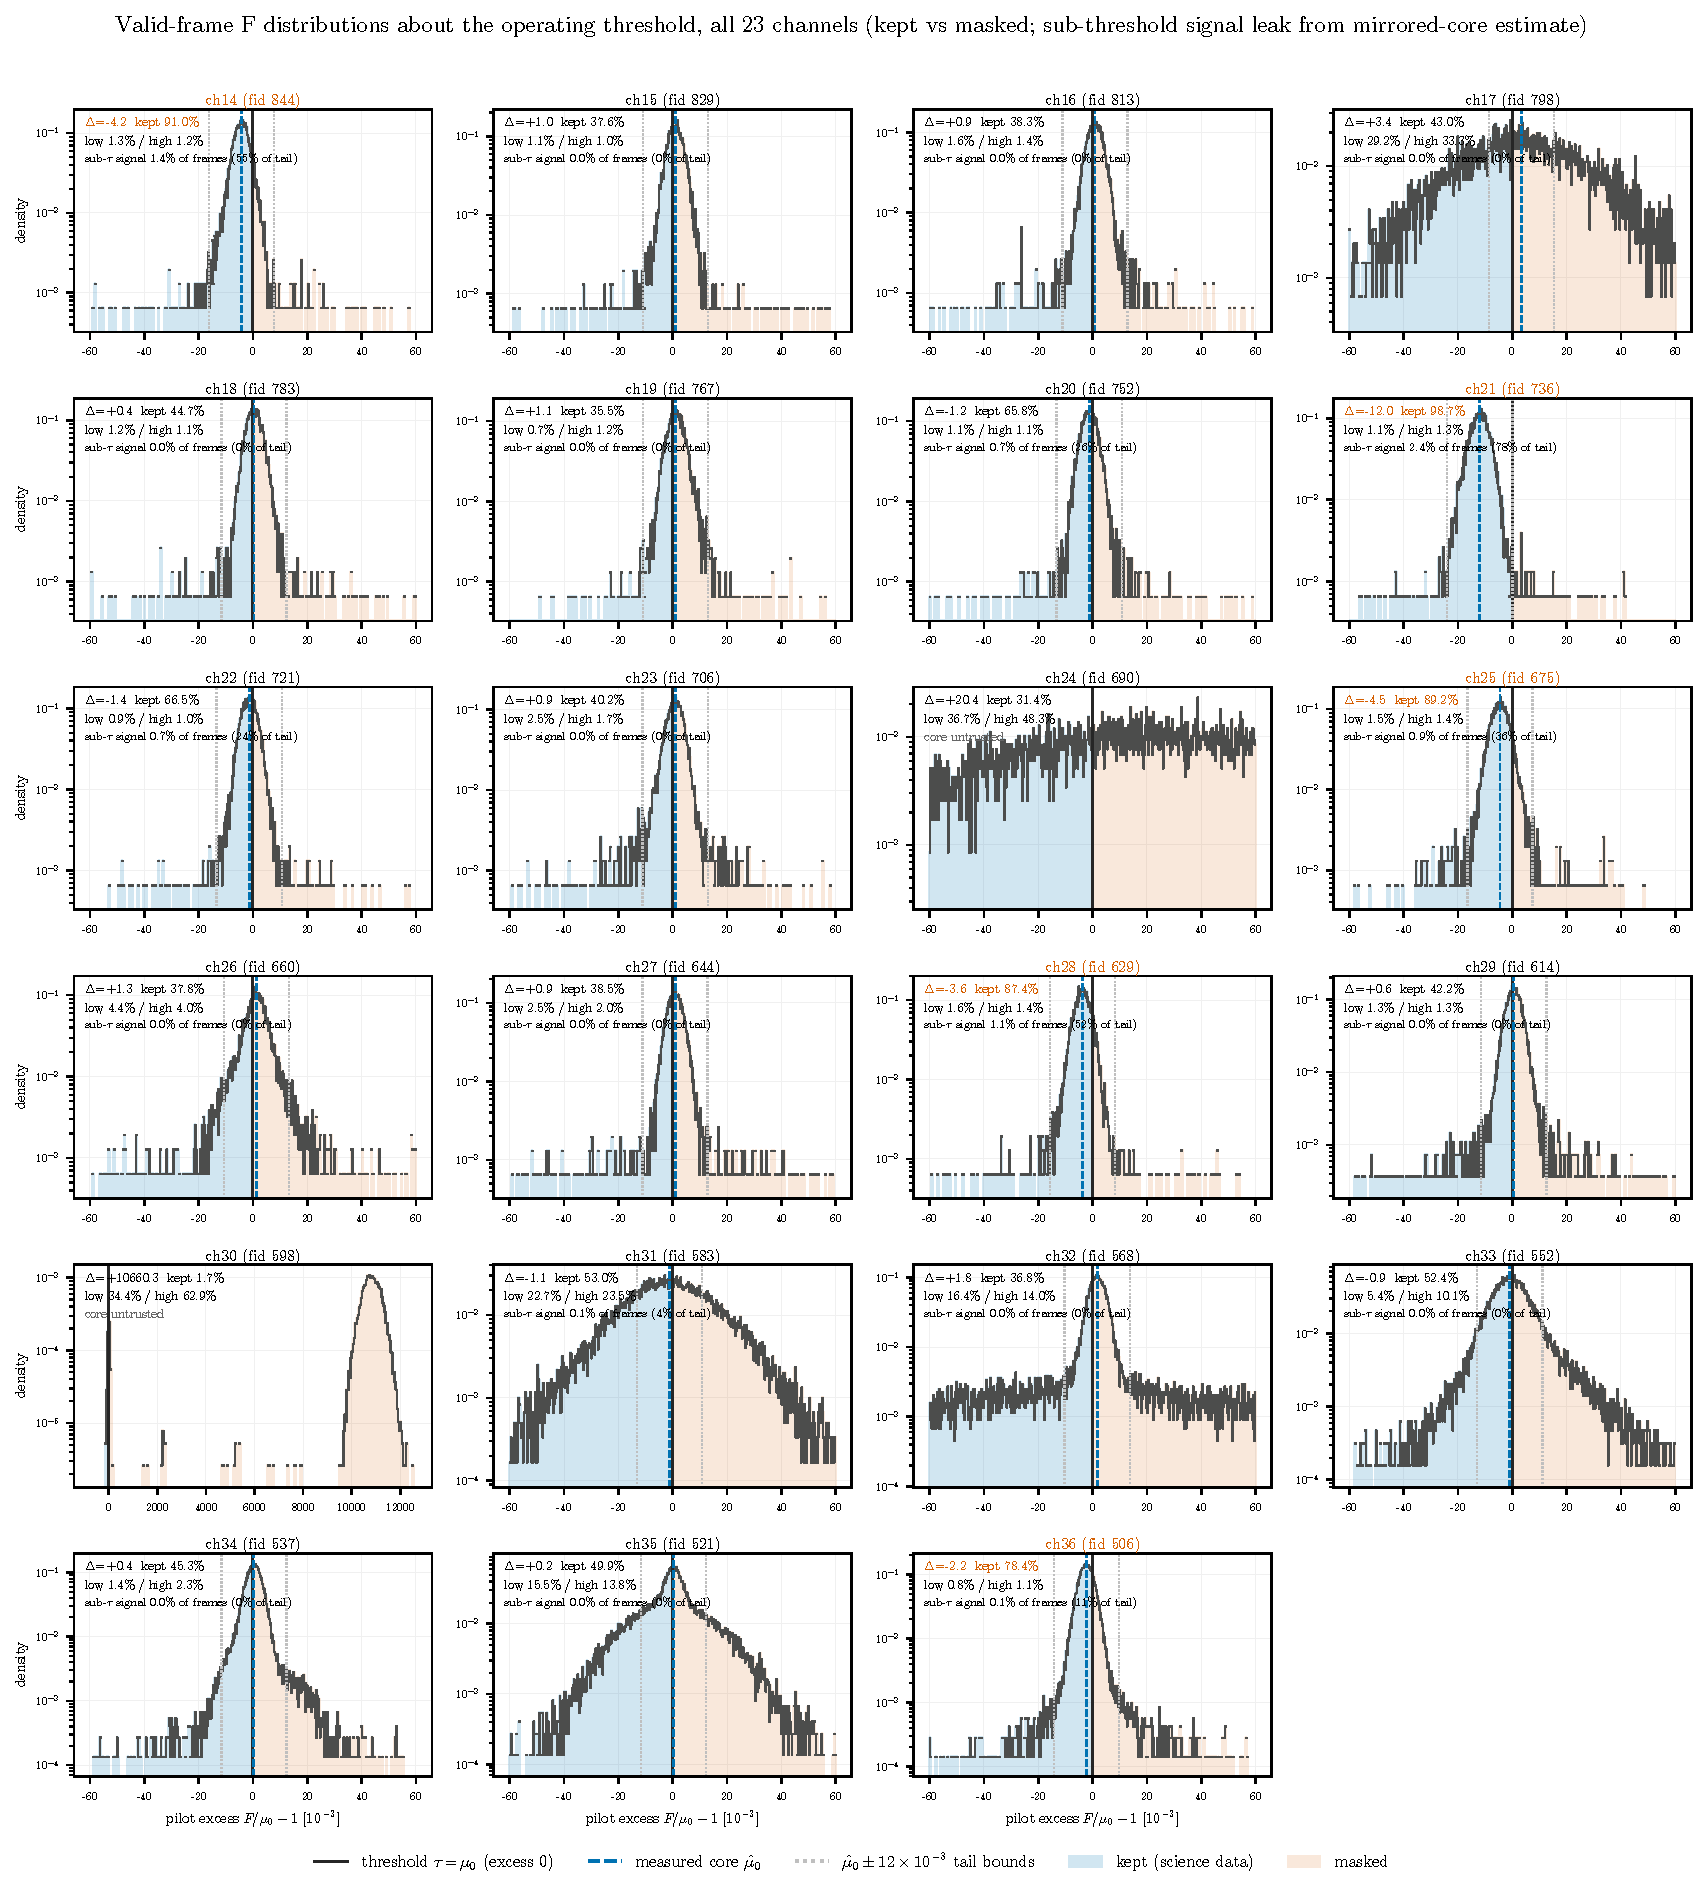
\includegraphics[width=0.94\textwidth]{fig_excess_threshold_all23}
\caption{Per-channel $F$ distributions about the operating threshold:
kept/masked split, both zero points, tail bounds, and the
sub-threshold leak estimate in a single view.}
\end{figure}
\begin{figure}[p]
\centering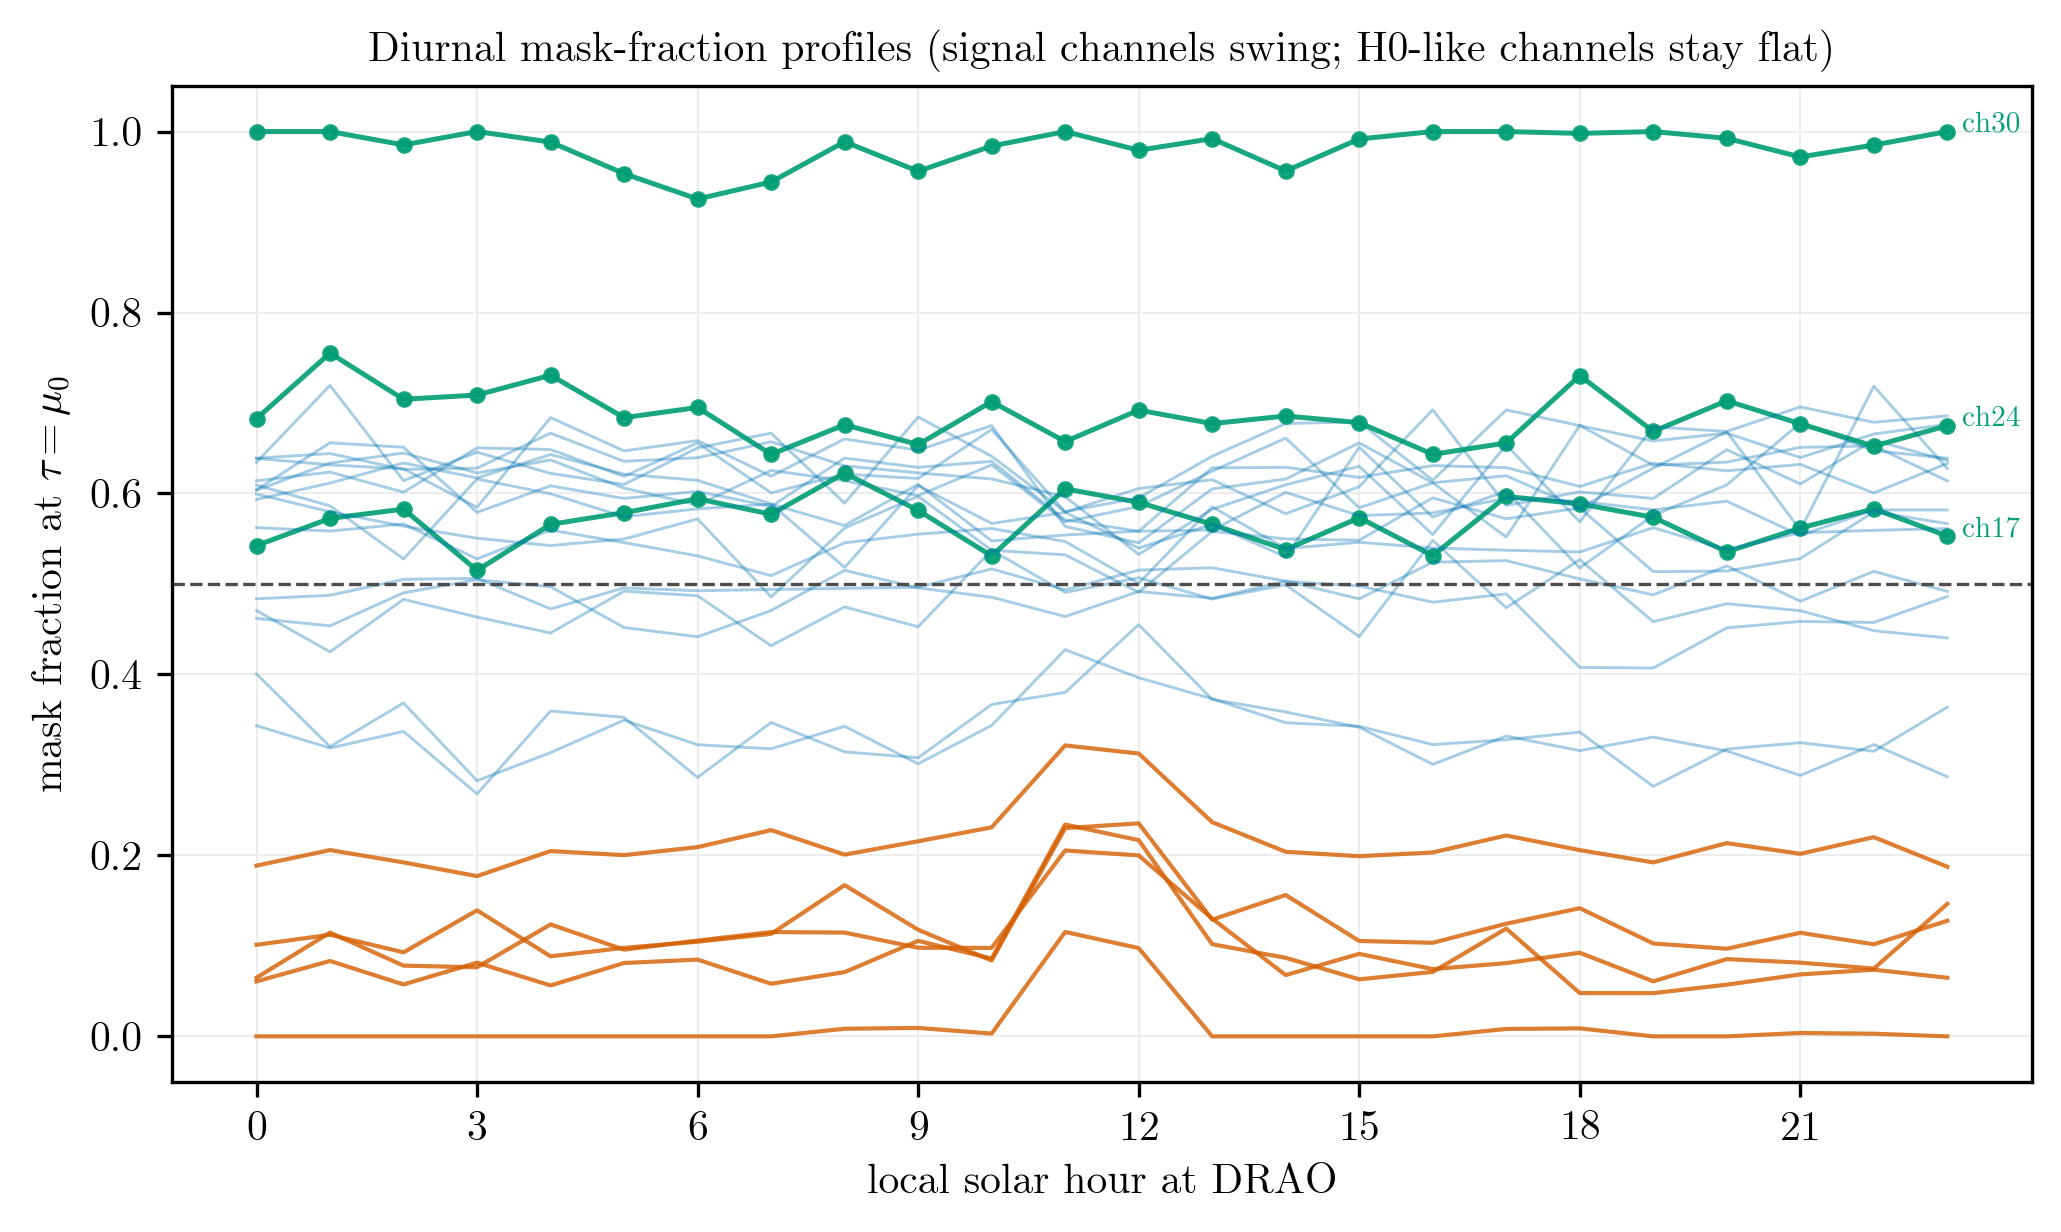
\includegraphics[width=0.86\textwidth]{fig_diurnal_mask_fraction}
\caption{Diurnal mask-fraction diagnostic.}
\end{figure}

\clearpage
\bigskip
\noindent\emph{Living-document note.} Sources for every section:
the public repository (\texttt{WVURAIL/pilot-proxy}), the archived
provenance memos (\texttt{DECISIONS}, \texttt{T2\_RESOLUTION},
\texttt{SURVEY\_COMPOSITION\_STRATUM}, \texttt{TIERING\_COMPLETENESS},
referee-triage series R5--R10), and the per-figure scripts named in
each section. New nuggets get appended as they are found; entries are
dated in the git history of this file.

\end{document}
